\section{Modelo de Diagrama de Interrelación de Documentos}

\subsection{DID}
Para poder satisfacer las consignas del enunciado, hemos diseñado el siguiente Modelo de Diagrama de Interrelación de Documentos.

\begin{center}
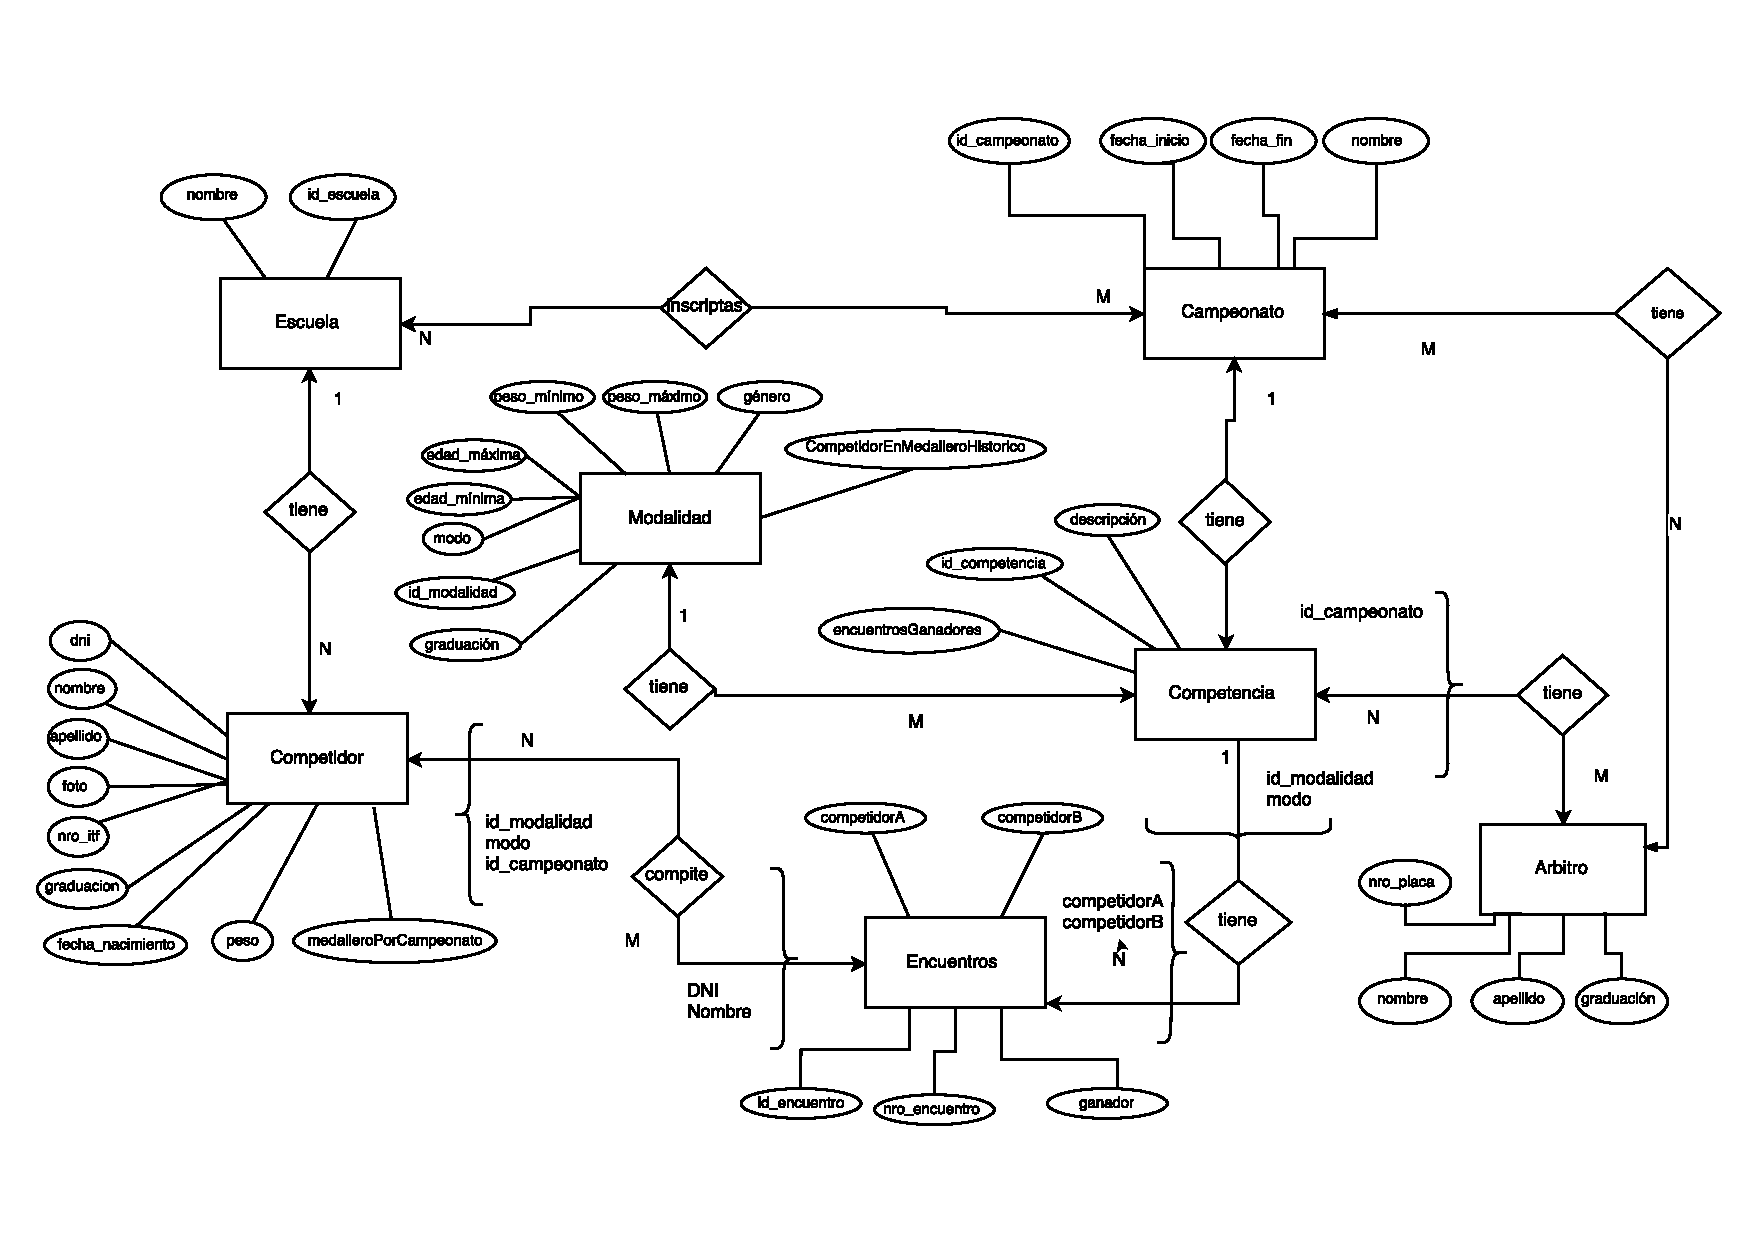
\includegraphics[width=11cm,keepaspectratio]{./imagenes/DID.pdf}\newline
\end{center}


\subsection{Entidades del DID}
A continuación, explicaremos diversas características de nuestro modelo, relacionando algunas entidades, y las funcionalidades que se obtienen de las mismas:

\subsubsection{Campeonato}

Esta entidad tiene los siguiente atributos:

\begin{itemize}
	\item id_campeonatos
	\item nombre
	\item fecha_inicio
	\item fecha_fin
\end{itemize}

y las siguientes relaciones:

\begin{itemize}
	\item escuelas
	\item arbitros
	\item competencias
\end{itemize}

 
De esta forma, estaremos cumpliendo con los siguientes requerimientos:

\begin{itemize}

	\item Historial de Competencias(funcionalidad extra 1): con la relación  ``competencias" , cada campeonato guardará la información de las competencia que hubo en ella.

	\item Historico de Arbitros(funcionalidad extra 3): guardamos la asociacion de los arbitros que participaran en cada campeonato.

	\item Historico de Escuela(funcionalidad extra 3): guardamos la asociacion de las escuelas inscriptas en el campeonato.

	\item Escuelas que participan, y la cantidad de participantes(funcionalidad 5).
	
\end{itemize}


\subsubsection{Competencia y Encuentro}

En el modelo del primer TP teníamos la relación entre Competencia y Competidor, y en ella
guardabamos el puesto que habia obtenido el competidor en ella. 
Ahora nos piden guardar la informacion de los encuentros, entonces, para cumplir con esta nueva especificación, tuvimos que modificar la relación descripta anteriormente y agregar una nueva entidad.

La entidad ``Encuentro", guardará la siguiente información:

\begin{itemize}
	\item id_encuentro
	\item nro_encuentro: número de encuentro en la competencia con la modalidad correspondiente.
	\item competidorA: id del competidor
	\item competidorB: id del competidor
	\item ganador: id del competidor ganador 
\end{itemize}

De esta manera guardaremos la información de cada encuentro y cada puesto obtenido(fucionalidad extra 2).

La entidad ``Competencia", guardará la siguiente información:

\begin{itemize}
	\item encuentrosGanadores: guarda por cada encuentro realizado en dicha competencia, quien ganó y quien perdió.
\end{itemize}

Con esta información podremos saber cuantos enfrentamientos ganó un competidor en una competencia, lo que premitirá saber cuantos ganó en un campeonato(funcionalidad 1).

\subsubsection{Competidor}

En esta entidad, agregamos dos nuevos atributos:
\begin{itemize}
	\item medalleroPorModalidad: contiene una lista con id de modalidades, en las que ganó una medalla.
	\item medalleroPorCampeonato: contiene una lista con id de campeonatos en las que ha participado.
\end{itemize}

Con esta información, se puede obtener el medallero de los campeonatos y las modalidades(funcionalidad extra 2).

\subsubsection{Modalidad}

Esta entidad, agregamos la siguiente información:

\begin{itemize}
	\item CompetidorEnMedalleroHistorico: indica los id's de los competidores que más medallas obtuvieron en dicha modalidad.
	\item cantMaximaMedallas: indica la cantidad de medallas que tienen los medalleros Históricos
\end{itemize}

Esta información permite rápida y eficientemente obtener los competidores que más medallas obtuvieron por modalidad(funcionalidad 6). La idea es que CompetidorEnMedalleroHistorico contiene la información, y cantMaximaMedallas permite mantener más fácilmente esta estructura. Asi pués, cada vez que se agregue una nueva competencia, hay que calcular quienes son los ganadores, agregarlos a los competidores, y usando las características de estos ver cuantas medallas tienen en esa modalidad:

\begin{itemize}
	\item Si tienen menos medallas que el máximo, no sucede nada.
	\item Si tienen la misma cantidad de medallas que el máximo, se los agrega a CompetidorEnMedalleroHistorico.
	\item Si pertenecían a CompetidorEnMedalleroHistorico, se borra la lista, se lo agrega a el, y se actualiza el máximo.
\end{itemize}


\subsubsection{Escuela}

Esta entidad, agregamos la siguiente información:

\begin{itemize}
	\item cantMedallasPorCampeonato: dice por cada campeonato cuantas medallas ganó la escuela.
\end{itemize}
 
 con esta información, se puede saber la cantidad de medallas por nombre de escuela en toda la historia(funcionalidad 2), sumando las medallas en cada campeonato, y para cada escuela, el campeonato donde ganó más medallas(funcionalidad 3). Para actualizar esta tabla, al ganar un competidor una competencia, se tiene que ver de que escuela es, y de que campeonato es la competencia, y sumarle 1 al campeonato correspondiente a la escuela.
 
\subsubsection{Arbitros}

Esta entidad, agregamos la siguiente información:

\begin{itemize}
	\item compeonatos: muestra los ids de los campeonatos en que participó.
\end{itemize}

Esta información nos permite saber en cuantos campeonatos y en cuales participó un arbitro(funcionalidad 4).